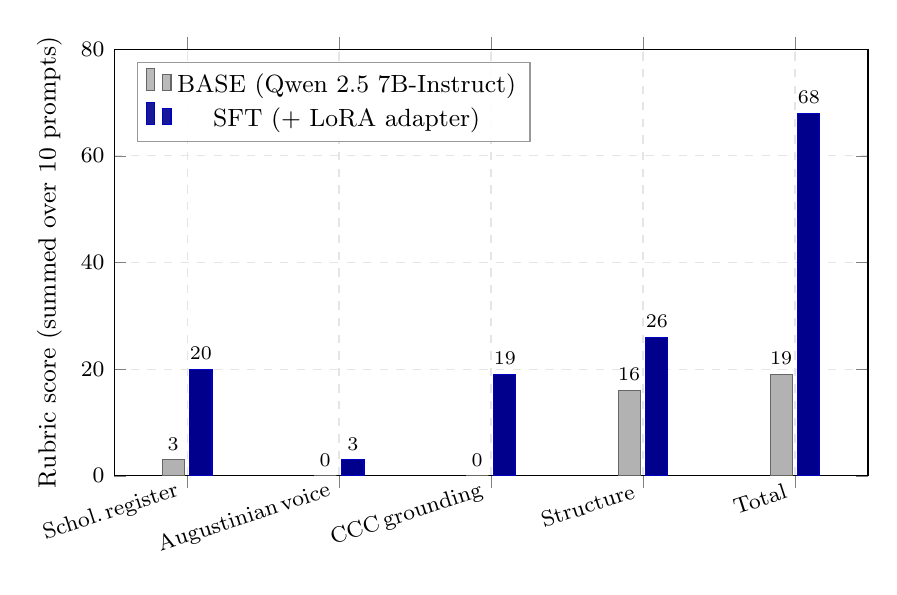
\begin{tikzpicture}
\begin{axis}[
    width=0.92\linewidth,
    height=7cm,
    ybar,
    bar width=8pt,
    ymin=0, ymax=80,
    enlarge x limits=0.12,
    ylabel={Rubric score (summed over 10 prompts)},
    symbolic x coords={Schol.\,register, Augustinian\,voice, CCC\,grounding, Structure, Total},
    xtick=data,
    x tick label style={font=\footnotesize, rotate=18, anchor=east},
    tick label style={font=\footnotesize},
    label style={font=\small},
    nodes near coords,
    nodes near coords style={font=\scriptsize},
    legend pos=north west,
    legend style={font=\small,fill=white,fill opacity=0.9,text opacity=1,draw=black!40},
    grid=major,
    grid style={dashed,gray!20},
  ]

  \addplot[fill=gray!60, draw=gray!80!black] coordinates {
    (Schol.\,register, 3)
    (Augustinian\,voice, 0)
    (CCC\,grounding, 0)
    (Structure, 16)
    (Total, 19)
  };
  \addlegendentry{BASE (Qwen 2.5 7B-Instruct)}

  \addplot[fill=blue!55!black, draw=blue!75!black] coordinates {
    (Schol.\,register, 20)
    (Augustinian\,voice, 3)
    (CCC\,grounding, 19)
    (Structure, 26)
    (Total, 68)
  };
  \addlegendentry{SFT (+ LoRA adapter)}

\end{axis}
\end{tikzpicture}
